\section{\centering L'apodisation}

\paragraph{Définition} Le but de l'\textbf{apodisation} est de "lisser" un signal assez brut afin d'enlever ou adoucir les discontinuités sur ses bords. 
Cela va permetttre d'augmenter le contraste et de supprimer en partie les anneaux de diffraction produits par les optiques, afin d'améliorer la définition des éléments à étudier, pour ce cas-ci la lumière de Proxima b.

\subsection{Bases sur la diffraction — Transformée de Fourier}

% \begin{itemize}
% \item La conversion pour comprendre comment on passe du plan pupille au plan focal
    
%     \item graphe largeur commune et tout, avec condition que la planete soit visible a tout les longueur d’onde et que la largeur commune soit plus grand que le coeur de la PSF a la longueur d’onde max 
% \end{itemize}


La \textbf{diffraction} est un phénomène qui se produit lorsqu'une onde rencontre un obstacle ou une ouverture. 

Prenons l'exemple classique du signal d'une étoile, que l'on considèrera comme une source ponctuelle à l'infini, passant à travers l'ouverture circulaire d'un téléscope. 

\begin{wrapfigure}[14]{r}{0.45\textwidth}
    \centering
    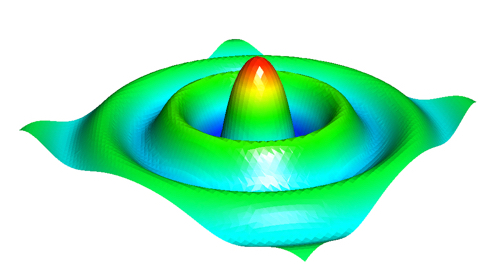
\includegraphics[width=0.4\textwidth]{figures/bessel_func.jpg}
    \caption{Fonction de Bessel d'ordre 1 $J_1$, aussi appelé "fonction sombrero".}
    \label{fig:sombrero}
\end{wrapfigure}

On part d'une onde plane à l'infini qui passe à travers une ouverture circulaire. Lorsque l'onde traverse ce plan, elle devient alors une fonction circulaire $\text{circ}_r(\rho')$ \ref{fig:diff_expl}.
En passant par cette ouverture, la fonction circulaire devient alors par transformée de Fourier la fonction de Bessel d'ordre 1 \ref{fig:sombrero}. Ce que l'on voit expérimentalement est une \textbf{tâche d'Airy}, correspondant à la fonction sombrero vue du dessus.

\begin{figure}[htbp]
    \centering
    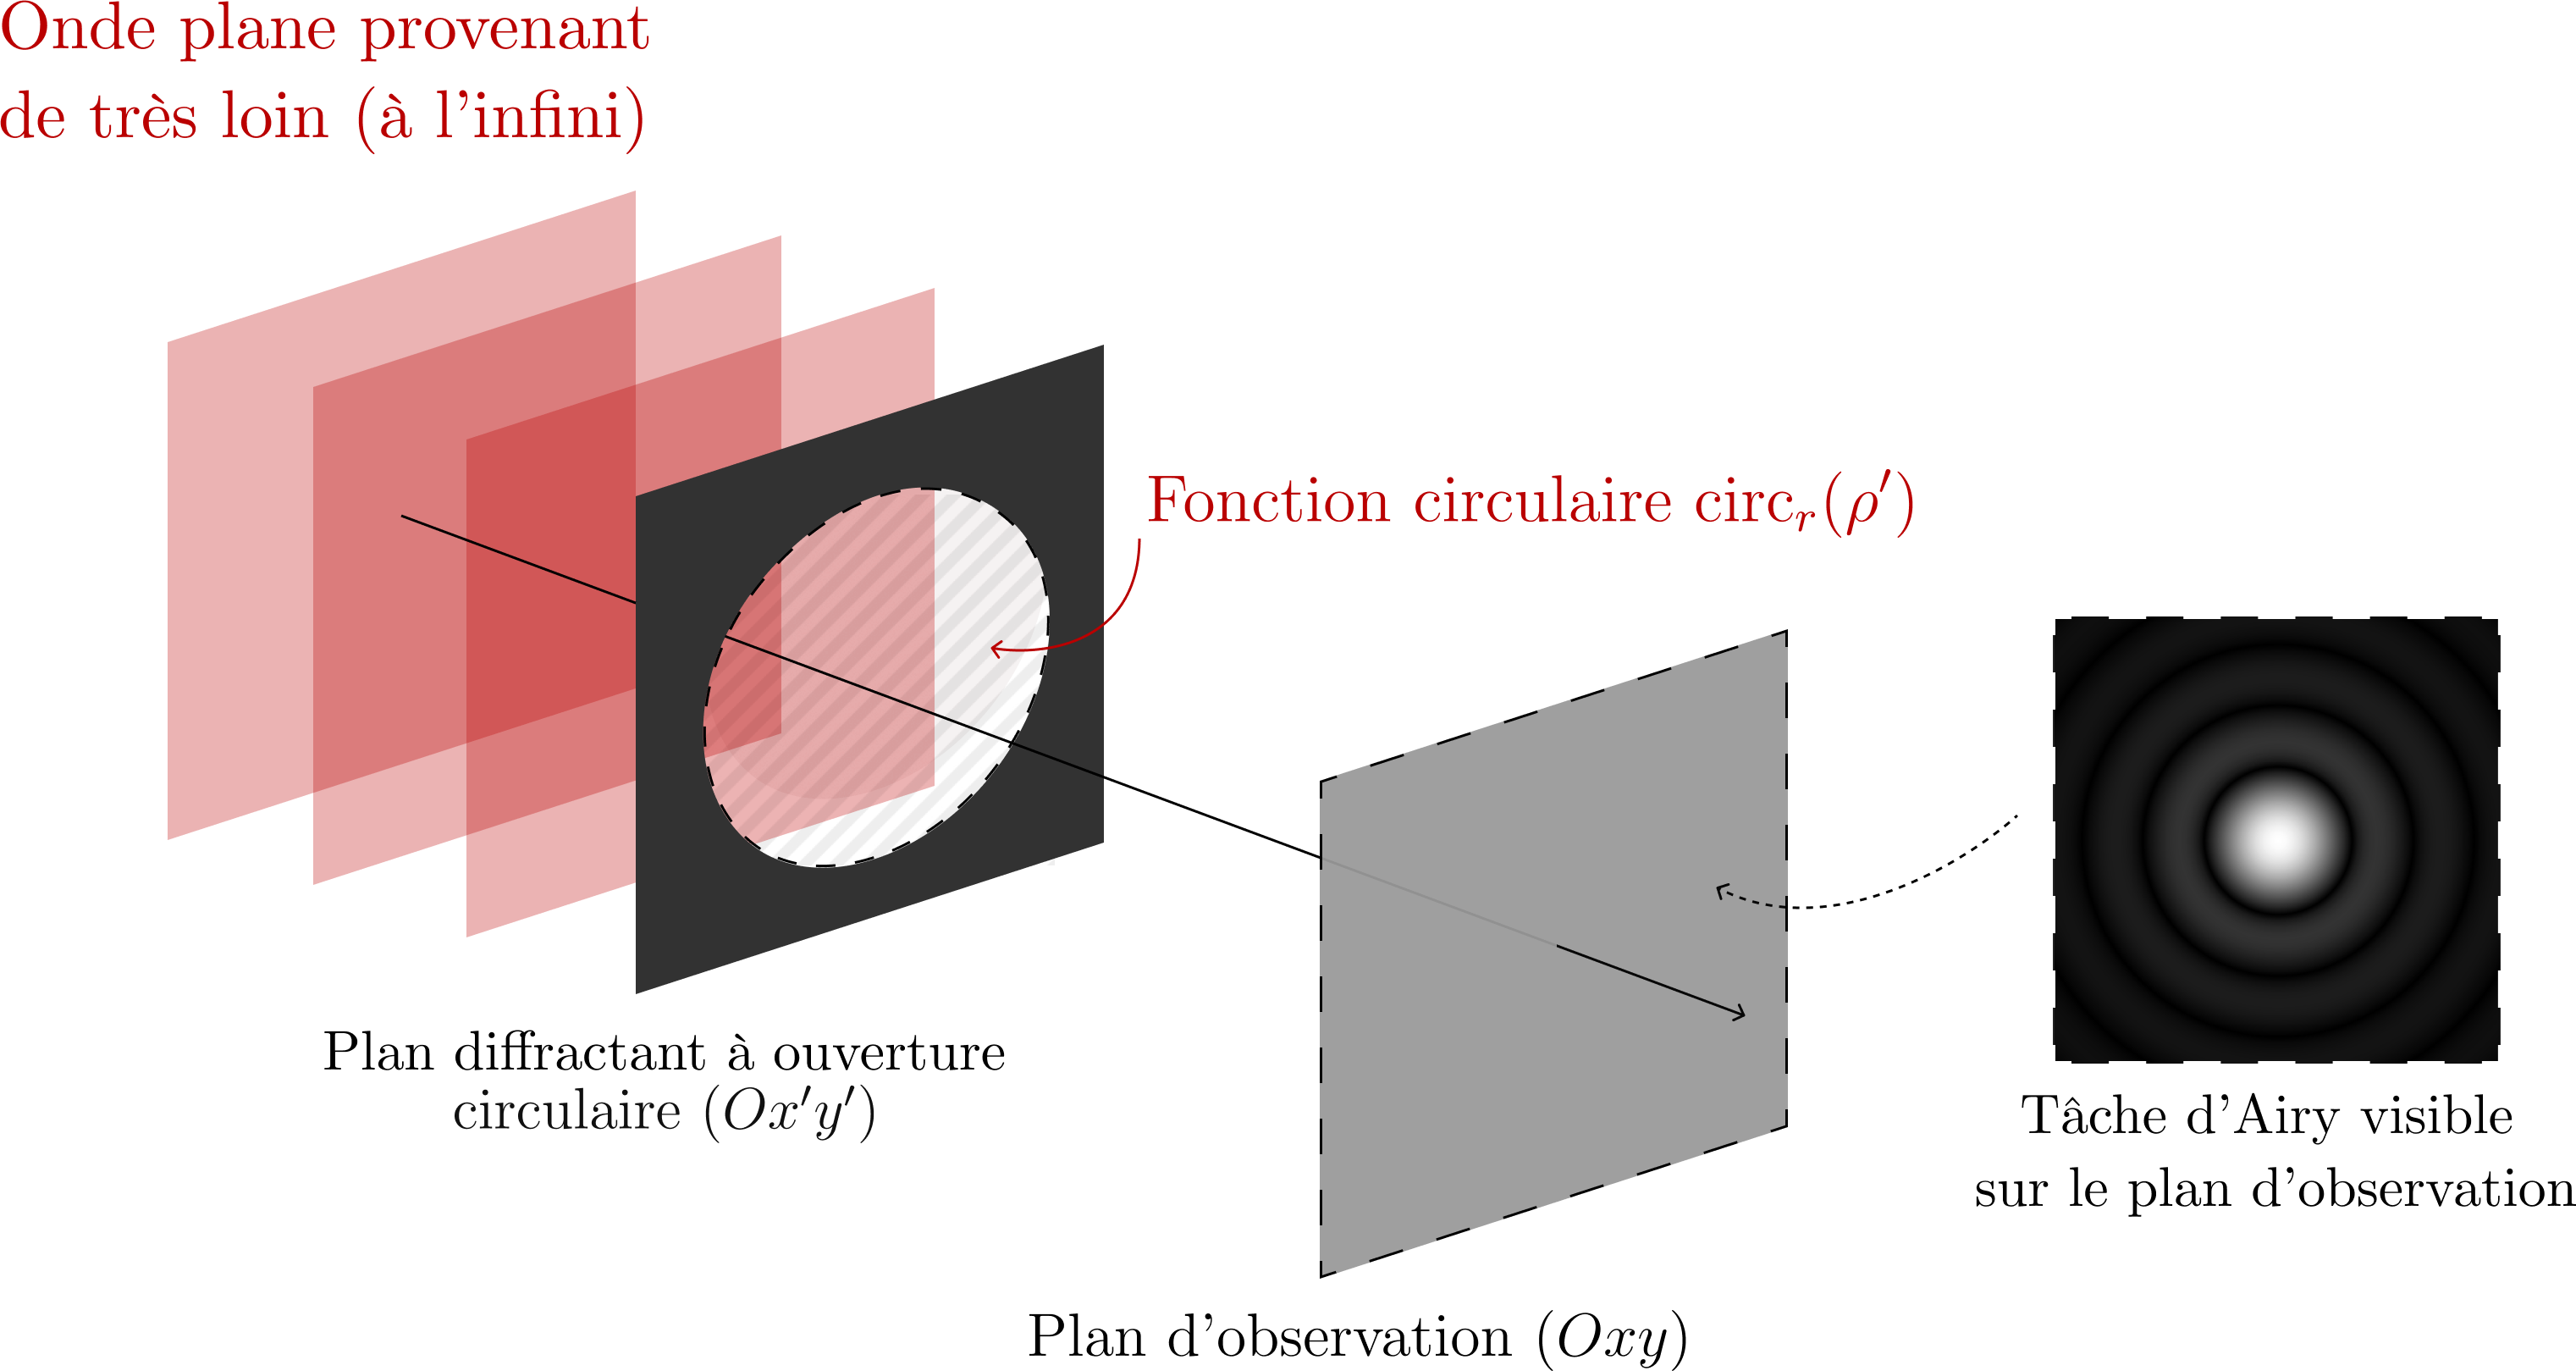
\includegraphics[width=0.75\textwidth]{figures/diff_expl.png}
    \caption{Diffraction d'une onde plane par une ouverture circulaire.}
    \label{fig:diff_expl}
\end{figure}

%\hspace*{3cm}

% \begin{figure}[htbp]
%     \centering
%     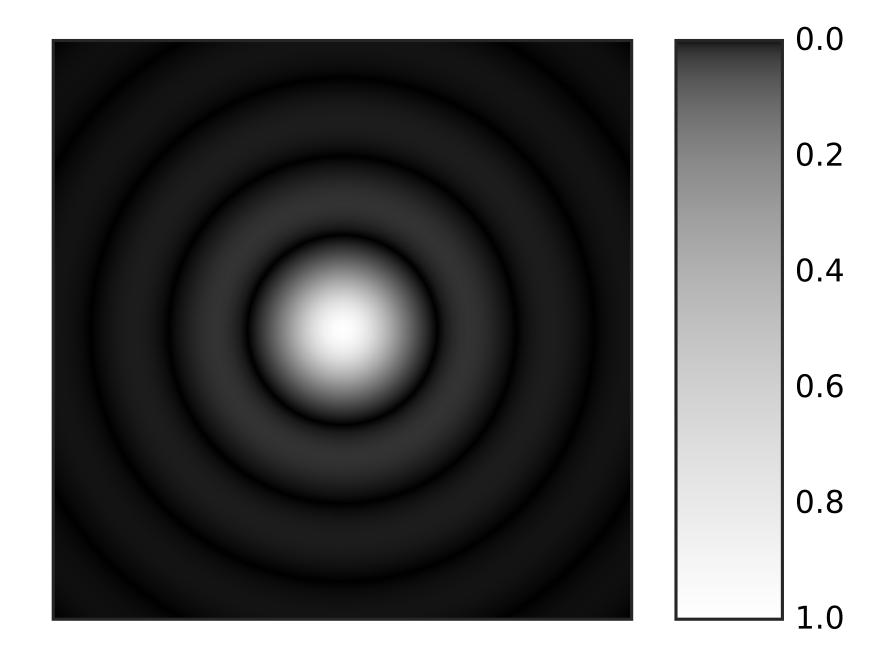
\includegraphics[width=\textwidth]{figures/airy_disk.png}
%     \caption{Tâche d'Airy. L'intensité maximum de la tâche est atteinte en son centre, où est concentré la majorité de l'énergie.}
% \end{figure}
%\caption{Comparaison entre la fonction sombrero et la tâche d'Airy. On remarque que la tâche d'Airy correspond à la vue de dessus de la fonction $J_1$}


Cette tâche d'Airy entraine que l’image d’un point ne peut pas être un point mais
va être une tâche proportionnelle au rayon de la tâche d’Airy, dont le rayon est proportionnel à $\lambda$.
Globalement, la tâche principale centrale (soit la lumière comprise dans le rayon $< 1.22\: \nicefrac{\lambda}{D}$) correspond à ce qu'on appelera le \textbf{coeur de la PSF} : l'essentiel de l'information que l'on peut récupérer de l'étoile se trouve dedans.

\begin{wrapfigure}[15]{l}{0.4\textwidth}
    \centering
    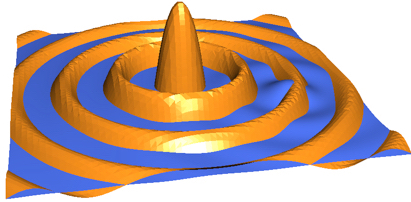
\includegraphics[width=0.4\textwidth]{figures/test_st_pl.jpg}
    \caption{Exemple de la tâche d'Airy d'une étoile et de son exoplanète proche, avec (a) montrant un signal à peu près distinguable et en (b) le signal de l'exoplanète encore plus faible que l'exemple (a), rendant impossible la récupération de l'information de la planète.}
\end{wrapfigure}

Ainsi, nous comprenons la nécessité de l'apodisation : la lumière diffracté de l'étoile va venir complétement recouvrir la lumière de l'exoplanète, rendant impossible l'analyse \iffalse ou genre récupérer l'information? \fi de la lumière de cette dernière. 

Afin de pouvoir créer une zone de haut contraste permettant l'observation d'une exoplanète proche de son étoile, différentes méthodes sont possibles : nous choisirons ici l’apodisation à l’aide d’un \textbf{masque pupille}. Nous commencerons par définir ce dont il s'agit.

\subsection{Masque pupille — Apodiseur}

Un \textbf{masque pupille} (aussi appelé \textbf{apodiseur}) est un carré en verre recouvert de chromium que l'on place dans le téléscope permettant de diffracter la lumière entrante dans le télescope de tel manière à pouvoir créer une zone où le contraste est suffisamment faible pour pouvoir observer des objets à luminosité très faibles autour d'objet très lumineux.  Leurs paramètres sont (1.) IWA, (2.) OWA, (3.) T, et (4.) potentiel forme de la dark zone

Ces masques permettent de diffracter la lumière autour de l’étoile afin de pouvoir créer une zone de haut contraste dans une zone souhaitée.

%Illustration of the apodization technique in the focalplane. Top left: unapodized amplitude split into two shiftedamplitude (bottom left). The result of this coherent additionis the first-apodized amplitude (top center). This approachcan be iteratively reproduced: the split and shifted amplitudes(bottom center) and second-apodized amplitude (top right).

\begin{figure}[htbp]
    \centering
    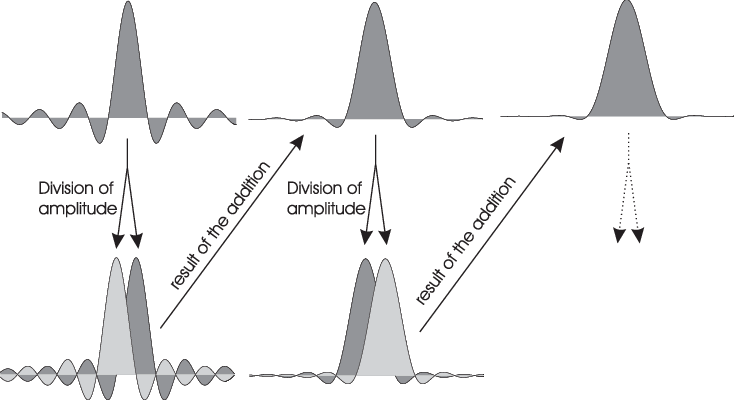
\includegraphics[width=0.7\textwidth]{figures/apod_explanation.png}
    \caption{Illustration de la technique d'apodisation dans le plan focal. En haut à gauche : amplitude non apodisée divisée en deux amplitudes décalées (en bas à gauche). Le résultat de cette addition cohérente est l'amplitude apodisée (en haut au centre). Cette approche peut être reproduite de manière itérative : les amplitudes divisées et décalées (en bas au centre) et l'amplitude apodisée (en haut à droite). }%\cite{apodExpl}}
\end{figure}

\begin{wrapfigure}[9]{l}{0.35\textwidth}
    \centering
    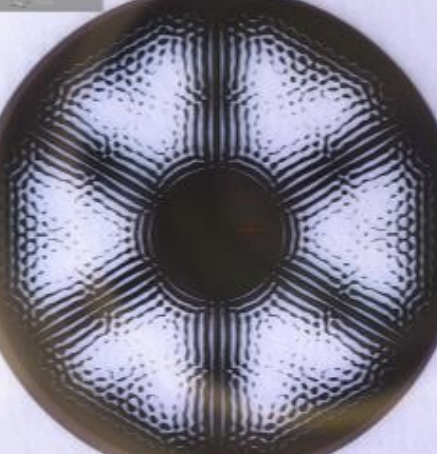
\includegraphics[width=0.30\textwidth]{figures/apod_harmoni.png}
    \caption{Apodiseur HC1 de l'instrument HARMONI.}%\cite{apod_harmoni}}
    %\label{fig:apod_harmoni}
\end{wrapfigure}

On peut ainsi remarquer qu'au fur et a mesure qu'on itère cette méthode, on crée une zone de haut contraste de plus en plus grande, permettant de récupérer de plus en plus d'information de l'exoplanète.



%Image montrant le principe physique de l'apodisation
Cependant, ce processus implique forcément une perte d'information, car la lumière de l'étoile est aussi diffractée. C'est pourquoi il est important de trouver un compromis entre la taille de la zone de haut contraste et la perte d'information.

En gros, on perd en résolution pour réduire la diffraction de l'étoile et augmenter le contraste de l'exoplanète.
% L’apodisation est une technique permettant de modifier la forme d’une fonction mathématique représentant un signal électrique, une transmission optique… de tel façon à enlever ou adoucir les discontinuités sur ces bords.
% Procédé destiné à augmenter le contraste et à supprimer, du moins en partie, les anneaux de diffraction produits par un instrument d'optique, afin d'améliorer la définition des éléments à étudier. [2.]

% L’apodisation est une technique permettant de modifier la forme d’une fonction mathématique représentant un signal électrique, une transmission optique… de tel façon à enlever ou adoucir les discontinuités sur ces bords.

% Procédé destiné à augmenter le contraste et à supprimer, du moins en partie, les anneaux de diffraction produits par un instrument d'optique, afin d'améliorer la définition des éléments à étudier. [2.]